\documentclass[a4paper,14pt]{extarticle} \usepackage[utf8]{inputenc}
\usepackage[T1]{fontenc}
\usepackage[margin=2.5cm]{geometry}

% Fonte Caladea se existir, senão lmodern
\IfFileExists{caladea.sty}{
  \usepackage{caladea}
}{
  \usepackage{lmodern} }
\usepackage{ragged2e}
\usepackage{graphicx}
\usepackage[portuguese]{babel}
\usepackage{wrapfig}
\usepackage{hyperref}
\usepackage{fancyhdr}
\usepackage{xcolor}
\usepackage{rotating}
\usepackage{titlesec}
\usepackage{epigraph}
\usepackage{dirtytalk}
\usepackage{indentfirst} % Indenta o primeiro parágrafo após seções

% Ajuste do recuo de parágrafo
\setlength{\parindent}{1.5em}

% Centralizar títulos
\titleformat{\section}
  {\normalfont\centering\bfseries\Large}{\thesection}{1em}{}

\titleformat{\subsection}
  {\normalfont\centering\bfseries\large}{\thesubsection}{1em}{}

\titleformat{\subsubsection}
  {\normalfont\centering\bfseries}{\thesubsubsection}{1em}{}

% -------------- Símbolos de Versículo e Resposta --------------
% Definição do símbolo (a “barrinha” inclinada)
\makeatletter
\newcommand{\vers@resp@sym}{%
  \raisebox{0.2ex}{\rotatebox[origin=c]{-20}{$\m@th\rceil$}}%
}
% macro interna que sobrepõe a barrinha e a letra V ou R
\newcommand{\vers@resp}[2]{%
  {\ooalign{%
     \hidewidth\kern#1\vers@resp@sym\hidewidth\cr
     #2\cr
  }}%
}
% comandos públicos \versicle e \response
\DeclareRobustCommand{\versicle}{\vers@resp{-0.1em}{V}}
\DeclareRobustCommand{\response}{\vers@resp{0pt}{R}}
\makeatother
% ^------------- Símbolos de Versículo e Resposta -------------^

% Rodapé com imagem e página
\pagestyle{fancy}
% ---- Cabeçalho ------------
\fancyhf[C]{}
% ----- Rodapé --------------
\fancyfoot[LO,LE]{%
  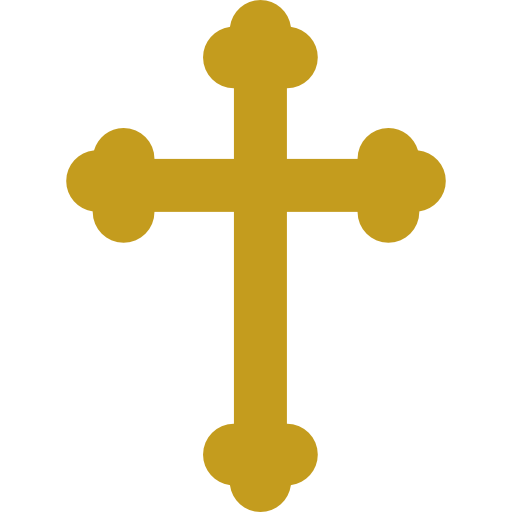
\includegraphics[scale=0.2]{assets/cross.png}\quad
  \textit{\textit{Sancte Regis Magi, orate pro Nóbis}}
}
\fancyfoot[RO,RE]{\thepage}

\usepackage{pdfpages}
\begin{document}
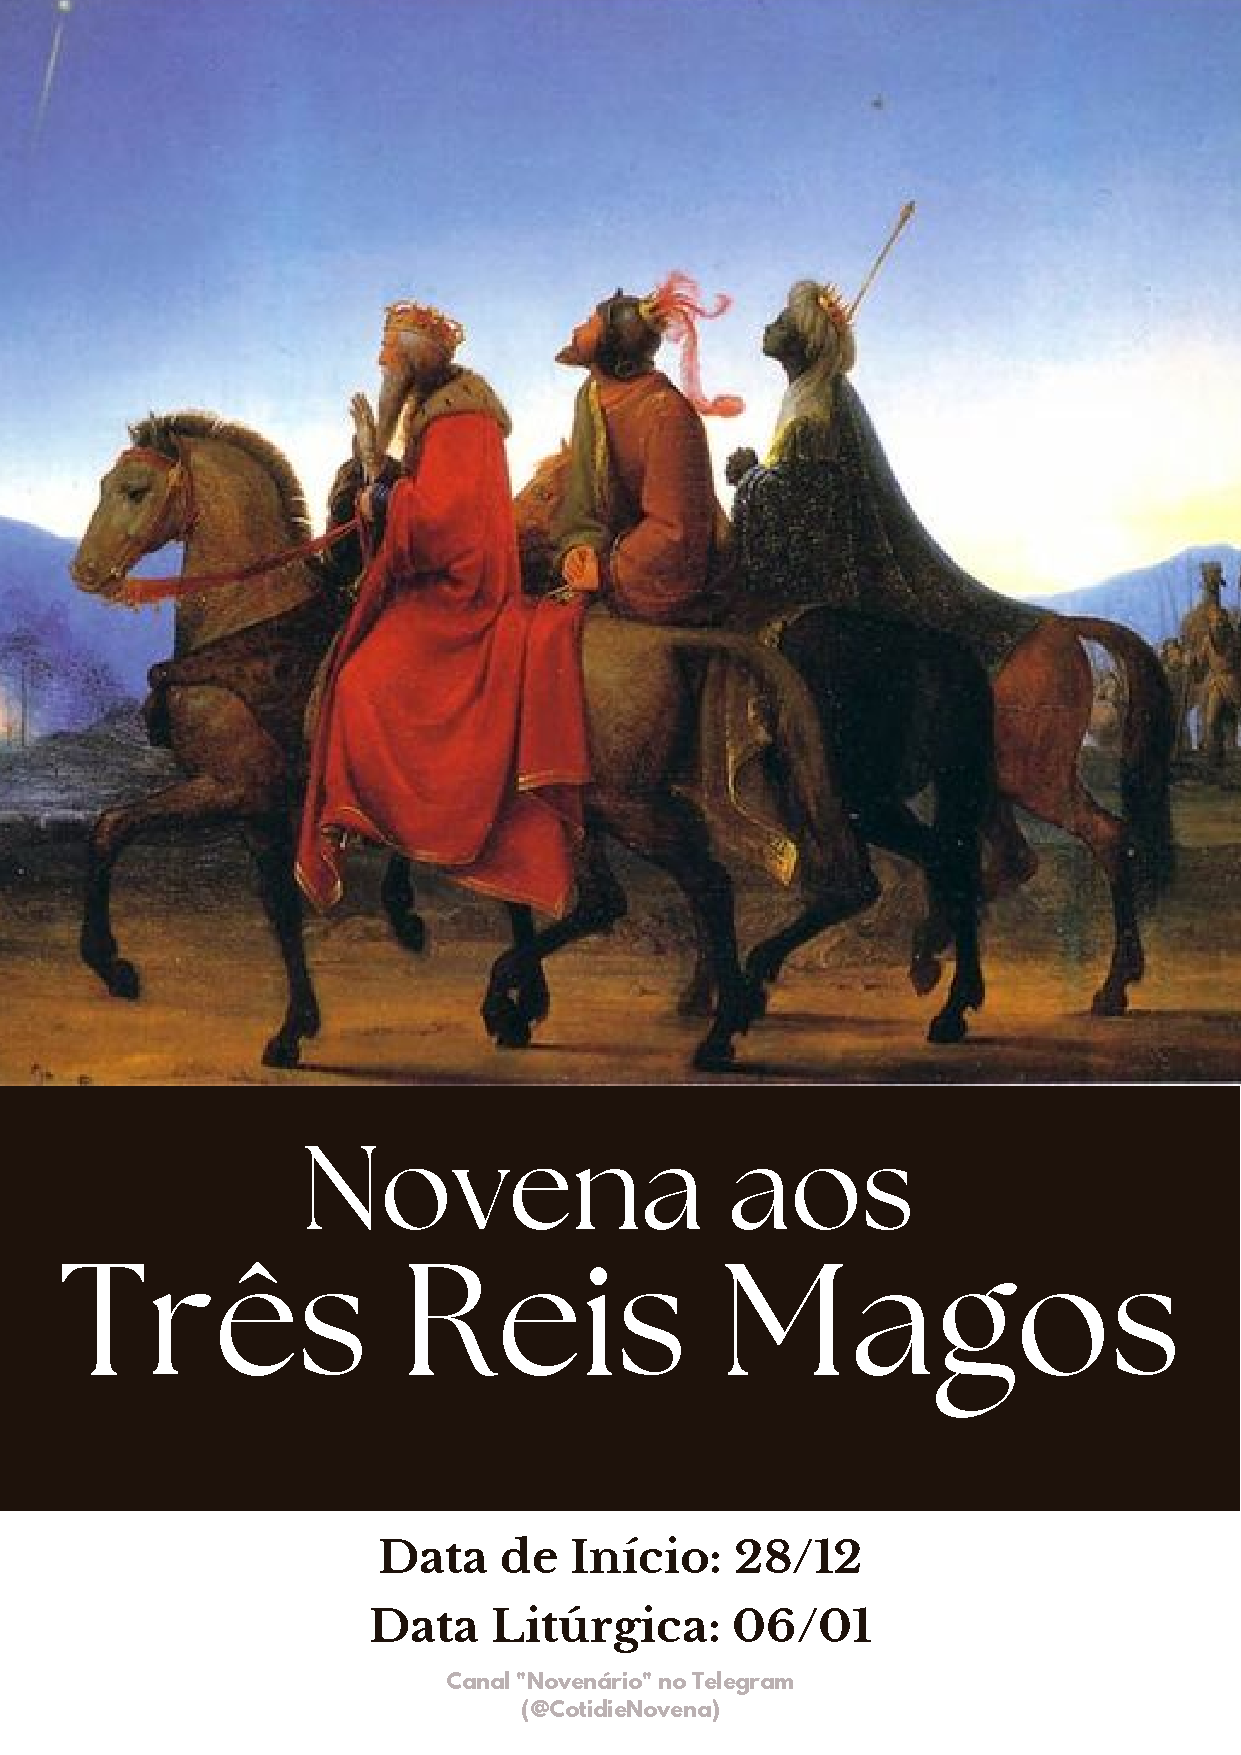
\includepdf[pages=1]{Capa Três Reis Magos.pdf}


\begin{center}
  {\huge Novena aos Três Reis Magos}
\end{center}


\say{Tendo pois nascido Jesus em Belém de Judá, tempo do rei Herodes, eis que uns magos vieram do Oriente a Jerusalém,
  dizendo: \say{Onde está o rei dos judeus, que acaba de nascer? Porque nós vimos a sua estrela no oriente, e viemos adorá-lo.}
Ao ouvir isto, o rei Herodes turbou-se, e toda (a cidade de) Jerusalém com ele.
E, convocando todos os príncipes dos sacerdotes e os escribas do povo, perguntou-lhes onde havia de nascer o Messias.
Eles disseram-lhe: \say{Em Belém de Judá, porque assim foi escrito pelo profeta:
E tu, Belém, terra de Judá, de modo algum és a menor entre as principais (cidades) de Judá, porque de ti sairá um chefe, que apascentará Israel, meu povo (Mq 5, 2).}}



\noindent\rule{\textwidth}{0.4pt}
\tableofcontents
\thispagestyle{empty}

% --- Vida / Origem da Novena ---
\newpage

% --- Orações Diárias ---
\newpage

\section{Os Reis Magos}
\subsection*{Quem foram os Reis Magos}

\textit{Evidências extra-bíblicas.} — Com base em evidências extra-bíblicas, é possível formular uma hipótese sobre o provável significado da palavra magoi. Heródoto (I 101) é a autoridade que nos leva a supor que os Magos eram a casta sagrada dos medos. Eles formavam os sacerdotes da Pérsia e, independentemente das vicissitudes dinásticas, sempre mantiveram a sua influência religiosa dominante. Ao chefe dessa casta, Nergal Sharezar, Jeremias dá o título de Rab-Mag, “Mago Chefe” (Jr 39, 3; 39, 13, no original hebraico — as traduções da Septuaginta; da Vulgata estão erradas nesse ponto). Após a queda do poder assírio e babilônico, a religião dos Magos dominou a Pérsia. Ciro conquistou completamente a casta sagrada, e seu filho Cambises a reprimiu severamente. Os Magos revoltaram-se e colocaram Gaumata, seu chefe, como rei da Pérsia sob o nome de Smerdis. No entanto, ele foi assassinado (521 a.C.), e Dario tornou-se rei. Essa queda dos Magos foi celebrada por um feriado nacional persa chamado magofonia (Heródoto III 63.73.79). Ainda assim, a influência religiosa dessa casta sacerdotal continuou durante todo o reinado da dinastia aquemênida na Pérsia (Ctesias, Persica, X-XV); e não é improvável que, na época do nascimento de Cristo, ela ainda estivesse florescendo sob o domínio parta. Estrabão (XI 9, 3) diz que os sacerdotes magos formavam um dos dois conselhos do Império Parta.

\textit{Evidências bíblicas.} — Tanto no Antigo como no Novo Testamento, a palavra magoi tem muitas vezes o significado de “mágico” (cf. At 8, 9; 13, 6; 8; Dn também a Septuaginta de 1, 20; 2, 2.10.27, 4, 4; 5, 7.11.15). São Justino (Tryph. 78), Orígenes (Cels. I 60), Santo Agostinho (Serm. 20, De Epiphania) e São Jerônimo (In Is. 19, 1) encontram o mesmo sentido no segundo capítulo de Mateus, embora não seja essa a interpretação comum.

\textit{Evidências patrísticas.} — Nenhum Padre da Igreja afirma que os Magos eram reis. Tertuliano (Adv. Marcion. III 13) diz que eles eram quase reis (fere reges), e assim concorda com o que concluímos a partir de evidências não-bíblicas. A Igreja, de fato, em sua liturgia, aplica aos Reis Magos as seguintes palavras: “Os reis de Társis e das ilhas oferecerão dons, os reis da Arábia e de Sabá trarão presentes; adorá-lo-ão todos os reis” (Sl 72, 10). Mas essa aplicação do texto a eles é tão incerta quanto sua viagem a partir de Társis, da Arábia e de Sabá. Como acontece às vezes, uma acomodação litúrgica de um texto acabou sendo considerada, com o tempo, uma interpretação autêntica do mesmo.

Tampouco eram mágicos: o sentido adequado de magoi, embora não se encontre em nenhuma outra parte da Bíblia, é exigido pelo contexto do segundo capítulo de São Mateus. Esses Magos só podem ter sido membros da casta sacerdotal já mencionada. A religião dos Magos era fundamentalmente a de Zoroastro e proibia a feitiçaria; foram a sua astrologia e a sua capacidade de interpretar sonhos que lhes permitiram encontrar o Cristo. O relato evangélico omite o número de Magos, e não existe uma tradição segura quanto a isso. Alguns Padres falam em três, muito provavelmente influenciados pelo número de presentes. No Oriente, a tradição prefere doze. A arte cristã primitiva não é um testemunho consistente: uma pintura no cemitério dos Santos Pedro e Marcelino mostra dois; outra que se encontra no Museu Lateranense, três; outra que está no cemitério de Domitila, quatro; um vaso do Museu Kircher, oito.

Os nomes dos Magos são tão incertos quanto o seu número. Entre os latinos, desde o século VII, encontramos ligeiras variantes dos nomes Gaspar, Melquior e Baltazar; o Martirológio antigo mencionava São Gaspar no dia 1.º, São Melquior no dia 6 e São Baltazar no dia 11 de janeiro (Acta Sanctorum I 8, 323.664). Os sírios têm Larvandad, Hormisdas, Gushnasaph etc.; os armênios, Kagba, Badadilma etc. (cf. Acta Sanctorum, Maio I, 1780). Deixando de lado a noção puramente lendária de que eles representavam as três famílias que descendem de Noé, todos eles parecem ter vindo “do Oriente” (cf. Mt 2, 1.2.9). A leste da Palestina, apenas a antiga Média, a Pérsia, a Assíria e a Babilônia tinham um sacerdócio como o dos Magos na época do nascimento de Cristo. Vieram eles de alguma dessas partes do Império Parta. Provavelmente atravessaram o deserto da Síria, situado entre o Eufrates e a Síria, chegaram a Haleb (Alepo) ou a Tudmor (Palmira), e viajaram para Damasco, na direção sul, por aquela que hoje é a grande rota de Meca (darb elhaj, “o caminho do peregrino”), mantendo o mar da Galileia e o Jordão a oeste até atravessarem o vau perto de Jericó.

Não existe tradição que defina com precisão o território designado por “o Oriente”. São Máximo (Homil. 18 in Epiphan.) e Teódoto de Ancira (Homil. de Nativitate I 10) afirmam que é a Babilônia; Clemente de Alexandria (Stromata I 15) e São Cirilo de Alexandria (In Is. 49, 12) dizem que é a Pérsia; São Justino (Cont. Tryphon. 77), Tertuliano (Adv. Jud. 9), e Santo Epifânio (Expos. fidei 8) dizem que é a Arábia.


\vfill

Leia mais em {\color{blue} \underline{\href{https://padrepauloricardo.org/blog/quem-foram-os-tres-reis-magos-e-quando-visitaram-jesus}{Padre Paulo Ricardo}.}}

\newpage

\section{Orações}

\subsection{1º Dia}

\say{Vê, a noite cobre a Terra, e a escuridão, os povos, mas sobre ti levanta-se o Senhor, e Sua glória te ilumina.} (Isaías 60,2). 

Ó Santos Magos, que vivestes em contínua espera da Estrela de Jacó, que viria a anunciar o Nascimento do verdadeiro Sol de Justiça, obtende-nos a graça de viver sempre na esperança de ver surgir sobre nós o dia da verdade, a beatitude do Paraíso. 

Reza-se a \textbf{\nameref{oracao-final}.}


\subsection{2º Dia}

\say{Levanta os olhos e olha à tua volta: todos se reúnem para vir a ti} (Isaías 60,4).  

Ó Santos Magos, que ao primeiro brilho da Estrela milagrosa abandonastes os vossos Países para ir à procura do Rei dos Judeus recém-nascido, obtende-nos a graça de corresponder prontamente, como vós, a todas as divinas aspirações. 

Reza-se a \textbf{\nameref{oracao-final}.}


\subsection{3º Dia}

\say{Os teus filhos chegam de longe, e tuas filhas são transportadas nos braços.}

Ó Santos Magos, que não temestes os rigores das estações nem os desconfortos da viagem para conseguirem encontrar o nascido Messias, obtende-nos a graça de não nos deixar jamais esmorecer diante das dificuldades que se encontram no caminho da Salvação.

Reza-se a \textbf{\nameref{oracao-final}.}


\subsection{4º Dia}

\say{As nações caminharão para à tua luz, e os reis, para o brilho de tua aurora.} (Isaías 60,3).

Ó Santos Magos, que, abandonados pela Estrela na cidade de Jerusalém, recorrestes com humildade e sem humano respeito a quem pudesse vos dar certa notícia do lugar onde se encontrava o objeto de vossas buscas, obtende-nos a graça de, em todas as dúvidas, em todas as perplexidades, nós recorrermos humildemente, e fielmente sigamos os conselhos dos nossos superiores que representam sobre a Terra a própria pessoa de Deus. 

Reza-se a \textbf{\nameref{oracao-final}.}


\subsection{5º Dia}

\say{Essa visão te tornará radiante; teu coração palpitará e se dilatará} (Isaías, 60,5).

Ó Santos Magos, que, contra toda vossa esperança, fostes novamente consolados pela Estrela que reapareceu para vos servir de guia, obtende-nos do Senhor a graça de, permanecendo a Ele fiéis em todas as aflições, mereçamos ser consolados por Sua graça, no tempo, e por Sua glória, na eternidade. 


Reza-se a \textbf{\nameref{oracao-final}.}



\subsection{6º Dia}

\say{... porque para ti afluirão as riquezas do mar, e a ti virão os tesouros das nações.} (Isaías, 60,5).

Ó Santos Magos, que, entrando cheios de fé no estábulo de Belém, prostrados à terra, adorastes o nascido Rei dos Judeus, ainda que não fosse cercado que pelos indícios de pobreza e fragilidade, obtende-nos do Senhor a graça de reavivar sempre a nossa Fé quando entrarmos em Sua casa, a fim lá habitarmos com aquele respeito que é devido à grandeza de sua Majestade. 


Reza-se a \textbf{\nameref{oracao-final}.}



\subsection{7º Dia}

\say{Serás invadida por uma multidão de camelos, pelos dromedários de Madiã e de Efá; virão todos de Sabá, trazendo Ouro e Incenso, e proclamando os louvores do Senhor.} (Isaías, 60,6).

Ó Santos Magos, que, oferecendo a Jesus Cristo Ouro, Incenso e Mirra, O reconhecestes concordes como Rei, como Deus e como Homem, obtende-nos do Senhor a graça de não nos apresentarmos nunca de mãos vazias diante d’Ele, mas que Lhe ofereçamos o Ouro da caridade, o Incenso da adoração e a Mirra da penitência, visto que sem essas virtudes é impossível encontrar o Seu agrado. 


Reza-se a \textbf{\nameref{oracao-final}.}


\subsection{8º Dia}

\say{Porque a nação ou o reino que recusar servir-te perecerá, e sua terra será devastada.} (Isaías, 60,12).

Ó Santos Magos, que, avisados por um Anjo para não voltar a Herodes, vos encaminhastes logo por outra estrada à vossa Pátria, obtende-nos do Senhor a graça de, após termos nos reconciliado com Ele nos Santos Sacramentos, vivamos apartados de tudo aquilo que poderia ser para nós ocasião de novos pecados.


Reza-se a \textbf{\nameref{oracao-final}.}


\subsection{9º Dia}

\say{Levanta-te, revista-te de luz, eis a tua Luz! A glória do Senhor se levanta sobre ti.} (Isaías, 60,1)

Ó Santos Magos, que, chamados os primeiros entre os Gentios ao conhecimento de Jesus Cristo, perseverastes até à morte na vossa profissão de Sua Fé, obtende-nos do Senhor a graça de sempre viver em conformidade com as promessas por Ele feitas no Santo Batismo, ou seja, de renunciar constantemente ao mundo e às suas pompas, à carne e às suas tentações, ao demônio e às suas sugestões, a fim de nos merecer como vós a visão beatifica daquele Deus que forma aqui na Terra o objeto de nossa Fé 


Reza-se a \textbf{\nameref{oracao-final}.}



\section{Oração Final} \label{oracao-final}

Glória ao Pai, ao Filho, e ao Espírito Santo... (3x)

Ó perfeitíssimos adoradores do recém-nascido Messias,
Santos Magos, verdadeiros modelos do cristão de coragem, 
Vós, que nada vos desanimou da árdua jornada. 
E que, prontamente, ao sinal da estrela, 
Seguistes as divinas aspirações, 
Obtende-nos do Senhor a graça de, à vossa imitação, 
Sempre ir a Jesus Cristo 
E de adorá-lO com viva Fé 
Quando entrarmos em Sua Casa. 

Fazei que Lhe ofereçamos continuamente
O Ouro da caridade, 
O Incenso da oração, 
A Mirra da penitência, 
E não declinemos jamais da estrada da santidade, 
Que Jesus nos ensinou tão bem com Seu próprio exemplo, 
Antes mesmo do que com Seus ensinamentos;

Fazei, ó Santos Magos, que possamos merecer do Divino Redentor
As Suas eleitas bênçãos aqui na Terra
E a imerecida posse, depois, da glória eterna. Amém. 

Em nome do Pai, do Filho, do Espírito Santo. Amém.

\[
\textbf{ Três Reis Magos, Rogai por nós! }
\]

\vfill

\begin{center}
\subsection*{Fontes:}
Adaptado de: {\color{blue} \underline{\href{https://precantur.blogspot.com/2018/12/novena-aos-rei-magos-ii.html}{Thesaurus Precum}}} e {\color{blue} \underline{\href{https://padrepauloricardo.org/blog/quem-foram-os-tres-reis-magos-e-quando-visitaram-jesus}{Padre Paulo Ricardo}.}} .
\end{center}


\end{document}
